%My thesis!
\documentclass[11pt,a4paper,titlepage]{report}
%\documentclass[a4paper,11pt,openright,twoside]{book}
\usepackage{amsmath}
\usepackage{ amssymb }
\usepackage{calligra}
\usepackage{amsfonts}
\usepackage[english]{babel}
\usepackage{verbatim}
\usepackage{indentfirst}
\usepackage{fancyhdr}
\usepackage{amsthm}
\usepackage{graphicx}
\usepackage{indentfirst}
\usepackage{microtype}
\usepackage{lmodern}
\usepackage{braket}
\usepackage{todonotes}

\usepackage[font=small,labelfont=bf]{caption}  %per la didascalia delle immagini
\usepackage{mathrsfs}  %per fare le lettere calligrafiche
\usepackage{bm}  %per mettere le lettere greche in grassetto
\usepackage[T1]{fontenc}     %pacchetto lettere accentate
\usepackage[utf8]{inputenc}   %pacchetto lettere accentate

\newtheorem*{remark}{Remark}

\newcommand{\HRule}{\rule{\linewidth}{0.5mm}}

% MER says: You can have no-indent later if you want to, but not while
% I'm reading this.
%\setlength\parindent{0pt} % toglie identazione ovunque
\usepackage[sc]{mathpazo}

\newcommand{\mesh}{\mathcal{T}_t}

% -----------------

\begin{document}

%--------------------------

\begin{titlepage}
%\begin{adjustwidth*}{10pt}{-40pt}
\begin{center}
\vspace*{-2.7cm}

\includegraphics{images/aquila_nome}
\\
\rule{\textwidth}{1pt}
\\[0.5cm]
{\Large DEPARTMENT OF MATHEMATICS}
\\[0.35cm]
{\Large MASTER DEGREE IN MATHEMATICS}
\\[2.3cm]
{\Large THESIS}
\\[1.5cm]
\textsc{\huge \textbf{Modeling and simulation of craniovertebral decompression}}
%\\[0.4cm]
%{\Large March 25th, 2015}
%\\[3cm]
\\[4.5cm]
\begin{minipage}{0.5\textwidth}
\flushleft {
\large Advisors: \\
 \textbf{Prof. Eleuterio F. Toro} \rule{0pt}{2.5ex}\\
 \normalsize University of Trento\\[0.4cm]
\large \textbf{Dr. Marie E. Rognes} \\
\large \textbf{Ms. Eleonora Piersanti} \\
\large \textbf{Dr. Victor Haughton} \\
 \normalsize Simula Research Laboratory\\[0.4cm] \rule{0pt}{2.5ex}}\\
\end{minipage}
\begin{minipage}{0.45\textwidth}
\flushright {\large
Student: \\
\rule{0pt}{2.5ex} \textbf{Carlo Cisale}\\
\normalsize University of Trento} \\
\end{minipage}

\vspace*{\fill}
{\Large ACADEMIC YEAR 2016-2017}
\rule{\textwidth}{1pt}


\end{center}
%\end{adjustwidth*}
\newpage
\thispagestyle{empty}
\phantom{}
\end{titlepage}
\newpage
\thispagestyle{empty}

%--------------------------

\tableofcontents
\pagenumbering{roman}

\newpage

\pagenumbering{arabic}

\chapter{Introduction}

\chapter{Medical background}

\chapter{Mathematical models}

\section{The Navier-Stokes equations}

\todo[inline]{Derivation of N-S equations?}

\subsection{The Navier-Stokes equations on a fixed domain}

% References:
% - Quarteroni
% - Vegard
% - Drosdal

The flow in the SAS and in the spinal cord can be described by the incompressible Navier-Stokes equations for Newtonian fluids. They describe the motion of a fluid with constant density $\rho$ in a domain $\Omega \subset \mathbb{R}^d$ (where $d=2,3$). They read

\begin{align}
\label{eq:ns:0}
\rho \dot{\mathbf{u}} + \rho (\mathbf{u} \cdot \nabla)\mathbf{u} - \nabla \cdot \sigma(\mathbf{u},p) &= \mathbf{f},  && \mathbf{x} \in \Omega, \, t>0 \\
\nabla \cdot \mathbf{u} &= 0, && \mathbf{x} \in \Omega, \, t>0
\end{align}

We are going to solve the problem for the velocity field $\mathbf{u}(\mathbf{x},t)$, and the pressure field $p(\mathbf{x},t)$, where $\mathbf{x} = (x,y)$. The quantity $\sigma(\mathbf{u}, p)$, is the Cauchy stress tensor for a Newtonian fluid, given by

\begin{equation}
\sigma(\mathbf{u}, p) = 2 \mu \epsilon(\mathbf{u}) - p \mathbb{I},
\end{equation}

where $\epsilon(\mathbf{u})$ is the symmetric strain rate tensor

\begin{equation}
\epsilon(\mathbf{u}) = \frac{1}{2} (\nabla \mathbf{u} + (\nabla \mathbf{u})^T).
\end{equation}

The constant $\mu$ represents the fluid viscosity, while $\mathbf{f}$ denotes a forcing term per unit of mass. Substituting $\sigma$ in~\eqref{eq:ns:0} we obtain

\begin{align}
\rho \dot{\mathbf{u}} + \rho ( \mathbf{u} \cdot \nabla) \mathbf{u} - \nabla \cdot [ \mu (\nabla \mathbf{u} + (\nabla  \mathbf{u})^T)] +  \nabla p &= \mathbf{f},  \\
\nabla \cdot \mathbf{u} &= 0,
\end{align}

The term $(\mathbf{u} \cdot \nabla)\mathbf{u}$ describes the process of convective transport, while $- \nabla \cdot [ \mu (\nabla \mathbf{u} + (\nabla  \mathbf{u})^T)] $ describes the process of molecular diffusion~\cite{}.\\
Since $\mu$ is constant, from the continuity equation we obtain

\begin{equation}
\nabla \cdot [ \mu (\nabla \mathbf{u} + (\nabla  \mathbf{u})^T)] = \mu [\Delta \mathbf{u} + \nabla(\nabla \cdot \mathbf{u})] = \mu \Delta \mathbf{u},
\end{equation}

hence the system can be written in the equivalent form

\begin{align}
\rho \dot{\mathbf{u}} + \rho ( \mathbf{u} \cdot \nabla) \mathbf{u} - \mu \Delta \mathbf{u} +  \nabla p &= \mathbf{f}, \\
\nabla \cdot \mathbf{u} &= 0.
\end{align}

In order for the problem to be well posed, it is necessary to assign an initial condition

\begin{equation}
\mathbf{u} (\mathbf{x}, 0) = \mathbf{u}_0(\mathbf{x}) \quad \forall \mathbf{x} \in \Omega,
\end{equation}

where $\mathbf{u}_0$ is a given divergence-free vector field, together with suitable boundary conditions, such as

\begin{align}
\mathbf{u}(\mathbf{x},t) &= \phi (\mathbf{x}, t) & \forall \mathbf{x} \in \Gamma_D \\
\left( \mu \frac{\partial \mathbf{u}}{\partial \mathbf{n}} - p\mathbf{n} \right) (\mathbf{x},t) &= \psi(\mathbf{x},t) & \forall \mathbf{x} \in \Gamma_N
\end{align}


where $\phi$ and $\psi$ are given vector functions, while $\Gamma_D$ and $\Gamma_N$ give a partition of the domain boundary $\partial \Omega$, that is $\Gamma_D 	\cup \Gamma_N = \partial \Omega, \mathring{\Gamma}_D \cap \mathring{\Gamma}_N = \emptyset$. Moreover, $\mathbf{n}$ is the outward unit normal vector to $\partial \Omega$. Equation in can also be written in another form

\begin{equation}
[ \mu (\nabla \mathbf{u} + \nabla \mathbf{u}^T)  - p\mathbf{n} ] = \psi(\mathbf{x}, t)  \quad \forall \mathbf{x} \in \Gamma_N.
\end{equation}

\begin{remark}
\normalfont{In our notation, if $\mathbf{u} = (u_x, u_y)^T$ and $\mathbf{x} = (x, y)^T$, then $\nabla \mathbf{u}$ is defined as

\[
\nabla \mathbf{u} =
\begin{pmatrix}
\frac{\partial u_x}{\partial x} & \frac{\partial u_x}{\partial y} \\
\frac{\partial u_y}{\partial x} & \frac{\partial u_y}{\partial y}
\end{pmatrix}
\]


}
\end{remark}


\subsection{Navier-Stokes on a moving domain}

Our next step is to allow the domain and its boundary to move, and
solve the Navier-Stokes equations on this deforming domain. Let
$\Omega^t$ denote the fluid domain which depends on time $t$. Let
$\Omega^0$ denote the fixed fluid domain at $t = 0$. In
fluid-structure interaction, the fluid domain $\Omega^t$ consists of
the same material particles at all times, and moves with the material
points within the structure. Also assume that we have a mesh $\mesh$
of the domain $\Omega^t$. Let $\mathbf{w}$ denote the \emph{mesh
  velocity}, and $\mathbf{y}$ the \emph{mesh displacement} with
respect to the reference domain $\Omega^0$, and thus by definition
$\dot{\mathbf{y}} = \mathbf{w}$ where the superposed dot denotes the
time derivative. The mesh velocity can be chosen arbitrarily in
principle, but this choice could effect the accuracy of the
solution~\cite{}.

The movement of the domain $\Omega^t$ is governed by the mesh
displacement, i.e.~for all $x(t) \in \Omega^t$, each corresponding to
a point $x_0 \in \Omega^0$, we have that
\begin{equation}
  x(t) = x_0 + \mathbf{y}(t)(x_0).
\end{equation}
\todo[inline]{Check the precise formulation carefully in Donea
  reference e.g.}

An ALE formulation of the Navier-Stokes equations on the deforming
domain $\Omega^t$ reads: find the velocity $\mathbf{u}$ and the
pressure $p$ such that
\begin{align}
  \label{eq:ns:1}
  \rho \dot{\mathbf{u}}
  + \rho [(\mathbf{u - w}) \cdot \nabla] \mathbf{u}
  - \mu \Delta \mathbf{u} + \nabla p
  &= \mathbf{f},  & \text{in } \Omega^t, \\
  \label{eq:ns:2}
  \nabla \cdot \mathbf{u} &= 0, & \text{in } \Omega^t,
\end{align}
for $t \in (0, T]$ where $\mathbf{f}$ is a given body force, $\rho$ is
  the fluid density, $\mu$ is the fluid viscosity. The
  system~\eqref{eq:ns:1}--\eqref{eq:ns:2} must be closed by
  appropriate boundary and initial conditions.

We will let the fluid domain boundary follow the changes on the
fluid-structure interface. Moreover, to move the entire domain, we
will use a \emph{Laplacian smoothing}
algorithm~\cite{Winslow1963}. More precisely, our mesh smoothing
equation reads: given a boundary velocity $\mathbf{u}_0$, find
$\mathbf{w}$ that satisfies
\begin{align}
\label{eq:bc:2}
- \Delta \mathbf{w} &= 0 	&& \text{in } \Omega^t, \\
\mathbf{w} &= \mathbf{u}_0 && \text{on } \partial \Omega^t .
\end{align}
\\
for each $t \in [0, T]$


\section{Modelling the SAS with elastic surroundings}

\begin{figure}
  \caption{Left: spinal cord in the SAS. Right: Schematic illustration
    of computational domain}
\end{figure}

We will consider a fluid domain $\Omega^t$ representing a section of
the subarachnoid space between the spinal cord and the surrounding
tissue.

Assuming axial symmetry along the spinal cord length axes, we consider
a two-dimensional rectangular reference domain $\Omega^0 = [0, L_x]
\times [0, L_y]$. We define the
\begin{itemize}
\item
  top boundary: $\partial \Omega_{\rm top}^0 = \{ (x_0, x_1) | x_1 = L_y\}$;
\item
  bottom boundary: $\partial \Omega_{\rm bottom}^0 = \{ (x_0, x_1) | x_1 = 0\}$;
\item
  tissue boundary: $\partial \Omega_{\rm tissue}^0 = \{ (x_0, x_1) | x_0 = L_x\}$;
\item
  cord boundary: $\partial \Omega_{\rm cord}^0 = \{ (x_0, x_1) | x_0 = 0\}$;
\end{itemize}
and thus $\partial \Omega^0 = \partial \Omega_{\rm top}^0 \cup
\partial \Omega_{\rm bottom}^0 \cup \partial \Omega_{\rm cord}^0 \cup
\partial \Omega_{\rm tissue}^0$. Further,
\begin{equation}
  \partial \Omega^t_{\rm i} = \partial \Omega^0_{\rm i} + \mathbf{y}(t)(\partial \Omega^0_{\rm i}),
\end{equation}
for each $i$.

We are interested in studying the effect of craniovertebral
decompression on the fluid flow and pressure dynamics in the
subarachnoid space. In particular, we assume that craniovertebral
decompression induces a change in the compliance of the tissue
surrounding the spinal canal~\cite{}. For simplicity, we aim to model
the compliance of the surrounding tissue via a boundary condition for
the fluid flow. We will assume that the tissue boundary $\partial
\Omega_{\rm tissue}$ is elastic with stiffness $k > 0$ and in particular
allowed to move. To this end, we introduce the boundary conditions
\begin{align}
\label{eq:bc:1}
(\mu \frac{\partial \mathbf{u}}{\partial \mathbf{n}} - p \mathbf{n}) \cdot \mathbf{n} = k \mathbf{y} \cdot \mathbf{n} \qquad \text{ on } \partial \Omega_{\rm tissue},\\
\label{eq:bc:3}
u^t = g = 0 \qquad \text{ on } \partial \Omega_{\rm tissue},
\end{align}

%\begin{equation}
%  \left ( \mu \nabla \mathbf{u} - p I
%  \right ) \cdot \mathbf{n} = \pm k \mathbf{y}
%  \qquad \text{ on }  \partial \Omega_{\rm tissue},
%\end{equation}

where $\mathbf{n}$ is the outward pointing boundary normal and
$\mathbf{y}$ still denotes the mesh displacement, and $u^t$ is the tangential component of the velocity field $\mathbf{u}$, i.e. $u^t = \mathbf{u} \cdot \mathbf{t}$. For simplicity, on
the spinal cord tissue, we assume that the cord is rigid and fixed,
i.e.:
\begin{equation}
  \mathbf{u} = \mathbf{0} \quad \text { on } \partial \Omega_{\rm cord}.
\end{equation}
% MER: Hmmm... This means that if y = 0, the wall is free to move.

To induce a fluid flow in the subarachnoid space, we impose the following condition on $\partial \Omega_{\rm tb} = \partial \Omega_{\rm top} \cup \partial \Omega_{\rm bottom}$ 

\begin{equation}
\label{eq:bc:6}
\mu \frac{\partial \mathbf{u}}{\partial \mathbf{n}} - p \mathbf{n} = -\bar{p} \mathbf{n}
\end{equation}

where $\bar{p}$ is a prescribed pressure. The inflow and outflow conditions are specified by the pressure function which we set up on the basis of chosen peak pressure and peak pressure gradient. We chose the maximum pressure during systole to be $1961Pa \approx 20 cmH_2O$ (Linge et. al., 2011 put reference). Moreover, we set the maximum difference in the pressure between the top and the bottom to be $24.3 Pa \approx 0.25 cmH_2O$ (water at $4^{\circ}$C). Since the CSF circulation is related to the cardiac cycle, during \textit{systole}, as blood flows into the brain, CSF flows down the Aqueduct of Sylvius. During \textit{diastole}, the opposite occurs. Hence, we choose the coordinate system so that the systolic flow is in negative $y$-direction, and while the diastolic flow is in the positive $y$-direction. We assume a heart rate of $60$ heart-beats per minute, so that the duration of the cardiac cycle is set to $1s$. The pressure functions is 

\begin{equation}
\bar{p}(y,t) = (a - \frac{y_{max} - y}{y_{max} - y_{min}}b) \cdot sin(2\pi t),
\end{equation}

where $t$ is the time, $a = 1961 Pa$, $b = 24.3 Pa$, and $y_{max}$ and $y_{min}$ denote the $y$-coordinate of the top and the bottom of the model. The sine term is added to reproduce the pulsatile motion of the fluid.

For the mesh equation, we let the mesh velocity follow the fluid
velocity on the tissue boundary, while the mesh velocity is assumed to
be zero (i.e.~the mesh boundary is fixed) on the remaining boundary:
\begin{align}
\label{eq:bc:5}
\mathbf{w} &= \mathbf{u}  \qquad \text{ on } \partial \Omega_{\rm tissue},\\
\mathbf{w} &= \mathbf{0}  \qquad \text{ on } \partial \Omega^t \setminus \partial \Omega_{\rm tissue}
\end{align}

In order to simplify the notation, in the following sections we are going to denote the moving domain $\Omega^t$ simply as $\Omega$. Moreover, note that $\partial \Omega_{\rm cord}$ and $\partial \Omega_{\rm
  tissue}$ are \textit{physical} boundaries, i.e.~they model portions
of the spinal cord and surrounding tissue. This means that
$\mathbf{u}$ and $\mathbf{w}$ should have the same value on these
boundaries, since the fluid follows the movement (if any) of the
walls.



\chapter{Numerical methods}

\section{Finite element formulation}

\section{Weak formulation of N-S on moving domain}
In order to obtain the weak formulation of the system~\eqref{eq:ns:1}--~\eqref{eq:ns:2}, we multiply the first equation by a test function $\mathbf{v}$ in a space $\hat{V}$ to be specified, and the second equation by a test function $q$ in a space $Q$, and integrate over $\Omega$. 
We obtain:

\begin{align}
\int_{\Omega} \rho \dot{\mathbf{u}} \, \mathbf{v} \, dx
+ \int_{\Omega} \rho [(\mathbf{u - w}) \cdot \nabla] \mathbf{u} \, \mathbf{v} \, dx
- \int_{\Omega} \nabla \cdot (\mu \nabla \mathbf{u} - pI)\mathbf{v} \, dx
&= \int_{\Omega} \mathbf{f} \mathbf{v} \, dx, \\
\int_{\Omega}  (\nabla \cdot \mathbf{u}) q \, dx &= 0.
\end{align}
\\
Integrating by parts the term $- \int_{\Omega} \nabla \cdot (\mu \nabla \mathbf{u} - pI)\mathbf{v} \, dx$, and applying Green formula, we have

\[
- \int_{\Omega} \nabla \cdot (\mu \nabla \mathbf{u} - pI)\mathbf{v} \, dx =  \int_{\Omega} (\mu \nabla \mathbf{u} - pI) \cdot \nabla \mathbf{v} \, dx - \int_{\partial \Omega} (\mu \nabla \mathbf{u} - pI) \cdot \mathbf{n} \, \mathbf{v} \, ds.
\]
\\
The space $\hat{V}$ is usually chosen such that the test function will be zero in the portion of the boundary were the solution is known. If $\Gamma_D$ is the portion of the boundary where we set Dirichlet conditions, we can define

\begin{equation}
\hat{V} = \set{\mathbf{v} \in [H^1(\Omega)]^2 | \mathbf{v}_{|_{\Gamma_D}} = \mathbf{0}} 
\end{equation}
\\
and we can choose $Q = L^2(\Omega)$. In our setup, the boundary $\partial \Omega$ is divided in the four boundaries:

\begin{equation}
\partial \Omega= \partial \Omega_{\rm top} \cup
\partial \Omega_{\rm bottom} \cup
\partial \Omega_{\rm cord} \cup
\partial \Omega_{\rm tissue}.
\end{equation}

Since we are assuming $\Gamma_D = \partial \Omega_{\rm cord}$, the test function $\mathbf{v}$ will be zero on this boundary. The boundary term becomes

\begin{equation}
\label{eq:bc:7}
\begin{split}
- \int_{\partial \Omega} (\mu \nabla \mathbf{u} - p I) \cdot \, \mathbf{n} \, \mathbf{v} \, dx =
-\int_{\partial \Omega_{\rm tb}} (\mu \nabla \mathbf{u} - p I) \cdot \, \mathbf{n} \, \mathbf{v} \, dx \\
- \int_{\partial \Omega_{\rm tissue}} (\mu \nabla \mathbf{u} - p I) \cdot \, \mathbf{n} \, \mathbf{v} \, dx.
\end{split}
\end{equation}
\\

From the boundary condition (\ref{eq:bc:6}), the term on the top and bottom boundaries in (\ref{eq:bc:7}) becomes

\begin{equation}
- \int_{\partial \Omega_{\rm tb}} (\mu \nabla \mathbf{u} - p I) \cdot \, \mathbf{n} \, \mathbf{v} \, dx = 
- \int_{\partial \Omega_{\rm tb}} (-\bar{p} \mathbf{n}) \cdot \, \mathbf{v} \, dx = 
\int_{\partial \Omega_{\rm tb}} \bar{p} \, \mathbf{n} \cdot \, \mathbf{v} \, dx
\end{equation}

Hence, the variational formulation reads:

\begin{equation}
\label{eq:ns:5}
\begin{split}
\int_{\Omega} \rho \dot{\mathbf{u}} \, \mathbf{v} \, dx
+ \int_{\Omega} \rho [(\mathbf{u - w}) \cdot \nabla] \mathbf{u} \, \mathbf{v} \, dx
+ \int_{\Omega} (\mu \nabla \mathbf{u} - pI) \cdot \nabla \mathbf{v} \, dx \\
+ \int_{\partial \Omega_{\rm tb}} \bar{p} \, \mathbf{n} \cdot \, \mathbf{v} \, dx
- \int_{\partial \Omega_{\rm tissue}} (\mu \nabla \mathbf{u} - p I) \cdot \, \mathbf{n} \, \mathbf{v} \, dx
=  \int_{\Omega} \mathbf{f} \mathbf{v} \, dx.
\end{split}
\end{equation}

As we are solving a Poisson equation for the mesh velocity $\mathbf{w}$, we need to discretize the problem. According to the boundary conditions~\eqref{eq:bc:5}, the function $\mathbf{w}$ belongs to the space

\begin{equation}
W = \set{\mathbf{w} \in [H^1(\Omega)]^2 | \mathbf{w}_{|_{\partial \Omega \setminus \Omega_{\rm tissue}}} = \mathbf{0}, \mathbf{w}_{|_{\partial \Omega_{\rm tissue} } }  = \mathbf{u} }.
\end{equation}

Let $\mathbf{z}$ be a test function in the space

\begin{equation}
\hat{W} = \set{\mathbf{z} \in [H^1(\Omega)]^2 | \mathbf{z}_{|_{\partial \Omega}} = \mathbf{0}}.
\end{equation}

\todo[inline]{Maybe somewhere I should say that the boundary $\partial \Omega$ depends on time and then I drop the $t$, otherwise I have too many t}


We multiply equation~\eqref{eq:bc:2} by $\mathbf{z}$ and integrate on the entire domain $\Omega$ to obtain

\begin{equation}
\label{eq:bc:4}
- \int_{\Omega} \Delta \mathbf{w} \, \mathbf{z} \, dx
= - \int_{\Omega} \nabla \mathbf{w} \cdot \nabla \mathbf{z} \, dx
+ \int_{\partial \Omega} \frac{\partial \mathbf{w}}{\partial \mathbf{n}} \mathbf{z} \, ds = 0.
\end{equation}
\\
Since $\mathbf{z} \in \hat{W}$, the term $\int_{\partial \Omega} \frac{\partial \mathbf{w}}{\partial \mathbf{n}} \, \mathbf{z} \, dx  = 0$. The final problem reads: find $\mathbf{w} \in W$ such that

\begin{align}
-  \int_{\Omega} \nabla \mathbf{w} \cdot \nabla \mathbf{z} \, dx &= 0, && \text{in } \Omega, \\
 \mathbf{w} &= \mathbf{u}, && \text{on } \partial \Omega_{\rm tissue}
\end{align}
for all $ \mathbf{z} \in \hat{W}$.


\subsection{The Nitsche method}
Our next step is to set the boundary conditions~\eqref{eq:bc:1} on the boundary $\partial \Omega_{\rm tissue}$. As we allow the tissue to move just in the normal direction, we need a way to set the tangential component of velocity field $\mathbf{u}$ to zero. In order to do so, we now give a brief introduction of a tool that allows us to impose boundary conditions in a weak way.

The Nitsche method was proposed as a way for treating boundary conditions in finite element method. In particular, it is used to weakly impose boundary and interface conditions, and it is applicable to a wide class of problems. Let us use Poisson's equation as a model problem. Given a domain $\Omega$ with boundary $\Gamma = \partial \Omega$, the problem is to find $\mathbf{u}$ such that

\begin{equation}
- \Delta \mathbf{u} = \mathbf{f} \qquad \text{ in } \Omega,
\label{eq:nitsche:1}
\end{equation}
subject to the boundary condition

\begin{equation}
\mathbf{u} = \mathbf{g} \qquad \text{ on } \Gamma.
\label{eq:nitsche:2}
\end{equation}

Generally, Dirichlet boundary conditions as~\eqref{eq:nitsche:2} are strongly imposed by seeking the solution $\mathbf{u}$ in some function space $V_g$, consisting of functions that already satisfy ~\eqref{eq:nitsche:2}. The idea of Nitsche's method~\cite{Nitsche1977} is to introduce a function space $V$ that does not satisfy that requirement, while 'weakly' enforcing the boundary condition. In order to derive the weak formulation, let us multiply equation~\eqref{eq:nitsche:1} by a test function $\mathbf{v}$ and integrate by parts. We obtain 

\begin{equation}
\label{eq:nitsche:3}
\int_{\Omega} \nabla \mathbf{u} \cdot \nabla \mathbf{v} \, dx
- \int_{\Gamma} \frac{\partial \mathbf{u}}{\partial \mathbf{n}} \cdot \mathbf{v} \, ds
= \int_{\Omega} \mathbf{f} \cdot \mathbf{v} \, dx. 
\end{equation}
We now want to enforce the boundary condition~\eqref{eq:nitsche:2} by adding a new term 

\begin{equation}
\int_{\Omega} \nabla \mathbf{u} \cdot \nabla \mathbf{v} \, dx
- \int_{\Gamma} \frac{\partial \mathbf{u}}{\partial \mathbf{n}} \, \mathbf{v} \, dx 
+ \int_{\Gamma} \mu (\mathbf{u} - \mathbf{g}) \cdot \mathbf{v} \, ds
= \int_{\Omega} \mathbf{f} \cdot \mathbf{v} \, dx,
\end{equation}

where $\mu$ is a  weight to adjust the penalty of the jump. Nitsche in ~\cite{Nitsche1977} proved that the choice $\mu = \gamma h^{-1}$, with $\gamma > 0$ a penalty parameter, and $h$ being the local mesh size, gives an optimally convergent method. In order to make the variational form symmetric, we can add the term $\int_{\Gamma} \frac{\partial \mathbf{u}}{\partial \mathbf{n}}(\mathbf{u}-\mathbf{g}) \, ds$. Hence, the final Nitsche method reads:

\begin{equation}
\begin{split}
\int_{\Omega} \nabla \mathbf{u} \cdot \nabla \mathbf{v} \, dx
- \int_{\Gamma} \frac{\partial \mathbf{u}}{\partial \mathbf{n}} \cdot \mathbf{v} \, ds
& - \int_{\Gamma} \frac{\partial \mathbf{v}}{\partial \mathbf{n}} \cdot \mathbf{u} \, ds 
+ \gamma \int_{\Gamma} h^{-1} \mathbf{u} \cdot \mathbf{v} \, ds = \\
	\int_{\Omega} \mathbf{f} \cdot \mathbf{v} \, dx
&- \int_{\Gamma} \frac{\partial \mathbf{v}}{\partial \mathbf{n}} \cdot \mathbf{g} \, ds
+ \gamma \int_{\Gamma} h^{-1} \mathbf{g} \cdot \mathbf{v} \, ds.
\end{split}
\end{equation}

We want to use the previous method to weakly set boundary conditions on the normal and the tangential components of the velocity field $\mathbf{u}$. The problem is to find $\mathbf{u}$ such that
\begin{align}
- \Delta \mathbf{u} &= \mathbf{f} \quad \text{ in } \Omega, \\
\label{eq:nitsche:4}
\frac{\partial \mathbf{u}}{\partial \mathbf{n}} \cdot \mathbf{n} &= l \quad \text{ on } \Gamma, \\ 
u^t &= g \quad \text{ on } \Gamma.
\end{align}
\\
where $\mathbf{u} = u^n \mathbf{n} + u^t \mathbf{t}$, and $\mathbf{n}$ and $\mathbf{t}$ are respectively the normal and tangential vectors. By substituting the test function $\mathbf{v} = v^n \mathbf{n} + v^t \mathbf{t}$ in~\eqref{eq:nitsche:3}, we obtain

\begin{equation}
\int_\Omega \nabla \mathbf{u} \cdot \nabla \mathbf{v} dx
- \int_{\Gamma} \frac{\partial \mathbf{u}}{\partial \mathbf{n}} (v^n \mathbf{n} + v^t \mathbf{t} ) \, ds
 = \int_\Omega \mathbf{fv} \, dx,
\end{equation}
\\
which leads to

\begin{equation}
\int_\Omega \nabla \mathbf{u} \cdot \nabla \mathbf{v} dx
- \int_{\Gamma}  \underbrace{ \frac{\partial \mathbf{u}}{\partial \mathbf{n}} \cdot \mathbf{n} }_{= l \text{ from} ~\eqref{eq:nitsche:4} }  v^n \, ds
- \int_{\Gamma} \frac{\partial \mathbf{u}}{\partial \mathbf{n}} \cdot \mathbf{t} v^t \, ds
= \int_\Omega \mathbf{f \cdot v} \, dx.
\end{equation}
\\
Applying the boundary condition~\eqref{eq:nitsche:4}, we have

\begin{equation}
\int_\Omega \nabla \mathbf{u} \cdot \nabla \mathbf{v} dx
-  \underbrace{ \int_{\Gamma} \frac{\partial \mathbf{u}}{\partial \mathbf{n}} \cdot \mathbf{t} \, v^t \, ds }_\text{Nitsche's method}
=  \int_{\Gamma} l \, v^n \, ds 
+ \int_\Omega \mathbf{f \cdot v} \, dx.
\end{equation}
\\
Applying the Nitsche method on the boundary term in the left hand side, we get

\begin{equation}
\begin{split}
\int_\Omega \nabla \mathbf{u} \cdot \nabla \mathbf{v} dx
- \int_{\Gamma} \frac{\partial \mathbf{u}}{\partial \mathbf{n}} \cdot \mathbf{t} \, v^t \, ds 
- \int_{\Gamma} \frac{\partial \mathbf{v}}{\partial \mathbf{n}} \cdot \mathbf{t} \, u^t \, ds
&+ \frac{\gamma}{h} \int_{\Gamma} u^t \, v^t \, ds \\
=  \int_{\Gamma} l \, v^n \, ds
+ \int_\Omega \mathbf{fv} \, dx.
- \int_{\Gamma} \frac{\partial \mathbf{v}}{\partial \mathbf{n}} \cdot \mathbf{t} \, g \, ds
&+ \frac{\gamma}{h} \int_{\Gamma} g \, v^t \, ds
\end{split}
\end{equation}

\subsection{Navier-Stokes formulation with the Nitsche method}
Finally, we apply what said earlier to the Navier-Stokes equations. Since $\nabla \mathbf{u} \cdot \mathbf{n} = \frac{\partial \mathbf{u}}{\partial \mathbf{n}}$, the boundary term in~\eqref{eq:ns:5} can be written as

\begin{equation}
\label{eq:ns:6}
\int_{\partial \Omega_{\rm tissue}} (\mu \nabla \mathbf{u} -  pI) \cdot \mathbf{n} \, \mathbf{v} \, ds
= \int_{\partial \Omega_{\rm tissue}} (\mu \frac{\partial \mathbf{u}}{\partial \mathbf{n}} -  p \mathbf{n}) \, \mathbf{v} \, ds \\ 
\end{equation}
\\
The vector $\mathbf{v}$ can be split in its normal and tangential components, i.e. $\mathbf{v} = v_n \mathbf{n} + v^t \mathbf{t}$. Substituting it in the term $(\mu \frac{\partial \mathbf{u}}{\partial \mathbf{n}} -  p \mathbf{n}) \, \mathbf{v}$, we have the following equalities:

\begin{align}
(\mu \frac{\partial \mathbf{u}}{\partial \mathbf{n}} -  p \mathbf{n}) \, \mathbf{v}
& = \mu \frac{\partial \mathbf{u}}{\partial \mathbf{n}} \cdot \mathbf{v} - p \, \mathbf{n} \cdot \mathbf{v} \\
& = \mu \frac{\partial \mathbf{u}}{\partial \mathbf{n}} \cdot (v_n \mathbf{n} + v^t \mathbf{t}) - p \, v_n \\
& = \mu \frac{\partial \mathbf{u}}{\partial \mathbf{n}} \cdot \mathbf{n} \, v_n + \mu \frac{\partial \mathbf{u}}{\partial \mathbf{n}} \cdot \mathbf{t} \, v^t   - p \, v_n \\
\label{eq:ns:7}
& = (\mu \frac{\partial \mathbf{u}}{\partial \mathbf{n}} - p\mathbf{n}) \cdot \mathbf{n} v_n + \mu \frac{\partial \mathbf{u}}{\partial \mathbf{n}} \cdot \mathbf{t} \, v^t. 
\end{align}

By integrating~\eqref{eq:ns:7} over $\partial \Omega_{\rm tissue}$, and from boundary condition~\eqref{eq:bc:1}, we obtain

\begin{equation}
\int_{\partial \Omega_{\rm tissue}} k \mathbf{y} \cdot \mathbf{n} \, v_n \, ds 
+ \underbrace{ \int_{\partial \Omega_{\rm tissue}} \mu \frac{\partial \mathbf{u}}{\partial \mathbf{n}} \cdot \mathbf{t} \, v^t \, ds }_{(\star)}
\end{equation}
\\
The last step is to apply Nitsche's method to the term $(\star)$, as shown in the previous section. Hence, the weak formulation of Navier-Stokes equations with Nitsche's method reads

\begin{equation}
\begin{split}
\label{eq:nitsche:6}
 \int_{\Omega} \rho \dot{\mathbf{u}} \, \mathbf{v} \, dx
+ \int_{\Omega} \rho [(\mathbf{u - w}) \cdot \nabla] \mathbf{u} \, \mathbf{v} \, dx
+ \int_{\Omega} (\mu \nabla \mathbf{u} - pI) \cdot \nabla \mathbf{v} \, dx \\
+ \int_{\partial \Omega_{\rm tb}} \bar{p} \, \mathbf{n} \cdot \, \mathbf{v} \, dx  % tob&bottom term
- \int_{\partial \Omega_{\rm tissue}} (k \mathbf{y}) \cdot \mathbf{n} v_n \, ds 
- \int_{\partial \Omega_{\rm tissue}} (\mu \frac{\partial \mathbf{u}}{\partial \mathbf{n}} \cdot \mathbf{t} \, v^t) \, ds \\
- \int_{\partial \Omega_{\rm tissue}} (\mu \frac{\partial \mathbf{v}}{\partial \mathbf{n}} \cdot \mathbf{t} \, u^t) \, ds
+ \frac{\gamma}{h} \int_{\partial \Omega_{\rm tissue}} u^t \, v^t \, ds \\
= \int_{\Omega} \mathbf{f} \mathbf{v} \, dx
- \int_{\partial \Omega_{\rm tissue}} (\mu \frac{\partial \mathbf{v}}{\partial \mathbf{n}} \cdot \mathbf{t} \, g) \, ds 
+ \frac{\gamma}{h} \int_{\partial \Omega_{\rm tissue}} g \, v^t \, ds
\end{split}
\end{equation}

Moreover, since we are assuming $u^t = g = 0$, the final form reads
\begin{equation}
\begin{split}
 \int_{\Omega} \rho \dot{\mathbf{u}} \, \mathbf{v} \, dx
+ \int_{\Omega} \rho [(\mathbf{u - w}) \cdot \nabla] \mathbf{u} \, \mathbf{v} \, dx
+ \int_{\Omega} (\mu \nabla \mathbf{u} - pI) \cdot \nabla \mathbf{v} \, dx \\
+ \int_{\partial \Omega_{\rm tb}} \bar{p} \, \mathbf{n} \cdot \, \mathbf{v} \, dx  % tob&bottom term
- \int_{\partial \Omega_{\rm tissue}} (k \mathbf{y}) \cdot \mathbf{n} v_n \, ds 
- \int_{\partial \Omega_{\rm tissue}} (\mu \frac{\partial \mathbf{u}}{\partial \mathbf{n}} \cdot \mathbf{t} \, v^t) \, ds \\
- \int_{\partial \Omega_{\rm tissue}} (\mu \frac{\partial \mathbf{v}}{\partial \mathbf{n}} \cdot \mathbf{t} \, u^t) \, ds 
+ \frac{\gamma}{h} \int_{\partial \Omega_{\rm tissue}} u^t \, v^t \, ds \\
= \int_{\Omega} \mathbf{f} \mathbf{v} \, dx
\end{split}
\end{equation}


\section{FEniCS}
\todo[inline]{Something about FEniCS}

\section{Numerical scheme}

\subsection{Time discretization}
In the following we present a discretization of the Navier-Stokes equations, that was used in the numerical simulations. Starting from equations~\eqref{eq:ns:1}--\eqref{eq:ns:2}, we want to use the so called Crank-Nicolson discretization to solve them. Let $[0, T] = \cup^N_{i=0} [t_i, t_{i+1}] $ be a time interval, and $\Delta t = t_{i+1} - t_i$ the time step. We apply a backward Euler discretization to the time derivative $\partial \mathbf{u}/ \partial t$

\begin{equation}
\frac{\partial \mathbf{u}}{\partial t} \approx \frac{\mathbf{u}^{i+1} -\mathbf{u}^i }{\Delta t},
\end{equation}
\\
where $\mathbf{u}^i$ is an approximation of $\mathbf{u}(t_i)$ at the time level $i$. A midpoint Crank-Nicolson scheme may be written as:

\begin{align}
\rho \frac{\mathbf{u}^{i+1} - \mathbf{u}^i}{\Delta t} + \rho [\nabla \mathbf{u} \cdot (\mathbf{u} - \mathbf{w})]^{i+1/2} - \nabla \cdot (\mu \Delta \mathbf{u}^{\rm  i+1/2} - p^{\rm i+1/2}I) &= \mathbf{f}^{\rm i+1/2}, \\
\nabla \mathbf{u}^{i+1} &= 0,
\end{align}
\\
where we set $\mathbf{u}^{\rm i+1/2} = \frac{\mathbf{u}^i + \mathbf{u}^{i+1}}{2}$.
The convective term may be written as

\begin{equation}
\rho [\nabla \mathbf{u} \cdot (\mathbf{u} - \mathbf{w})]^{i+1/2} = \rho [\nabla \mathbf{u}^{i+1/2} \cdot (\mathbf{u}^{i+1/2} - \mathbf{w}^{i+1/2})].
\end{equation}
We linearize the term above with

\begin{equation}
\rho [\nabla \mathbf{u}^{i+1/2} \cdot (\mathbf{u}^{i+1/2} - \mathbf{w}^{i+1/2})] \approx \rho [\nabla \mathbf{u}^{i+1/2} \cdot (\mathbf{u}^i - \mathbf{w}^i)].
\end{equation}
Moreover, the stress tensor $\sigma$ is discretized as follows 

\begin{equation}
\nabla \cdot \sigma \approx \nabla \cdot \sigma^i = \nabla \cdot (\mu \Delta \mathbf{u}^{\rm i+1/2} - p^{\rm i+1/2} I).
\end{equation}
The resulting discretization yields to

\begin{align}
\rho \frac{\mathbf{u}^{i+1} - \mathbf{u}^i}{\Delta t} + \rho [\nabla \mathbf{u}^{i+1/2} \cdot (\mathbf{u}^i - \mathbf{w}^i)] - \nabla \cdot (\mu \Delta \mathbf{u}^{\rm  i+1/2} - p^{\rm i+1/2}I) &= \mathbf{f}^{\rm i+1/2}, \\
\nabla \mathbf{u}^{i+1} &= 0,
\end{align}
\\
By defining the inner products

\[
\langle f, g \rangle_\Omega = \int_\Omega f \cdot g \, d \Omega, \qquad
\langle f, g \rangle_\Gamma = \int_\Omega f \cdot g \, d \Omega_{\rm tissue},
\]
\\
the numerical scheme reads

\begin{equation}
\begin{split}
\rho \langle \frac{\mathbf{u}^{\rm i+1} - \mathbf{u}^{\rm i}}{\Delta t}, \mathbf{v} \rangle_\Omega
+ \rho \langle \nabla \mathbf{u}^{\rm i+1/2} \cdot (\mathbf{u}^{\rm i} - \mathbf{w}^{\rm i}), \mathbf{v} \rangle_\Omega
+ \mu \langle \nabla \mathbf{u}^{i+1/2} , \nabla \mathbf{v} \rangle_\Omega
& - \langle p , div(\mathbf{v}) \rangle_\Omega \\
- \langle q , div \, \mathbf{u}^{\rm i+1} \rangle_\Omega
- \mu \langle (\nabla \mathbf{u}^{i+1} \cdot \mathbf{n}) \cdot \mathbf{t} , v^t \rangle_\Gamma 
- \mu \langle (\nabla \mathbf{v} \cdot \mathbf{n}) \cdot \mathbf{t} , u^t \rangle_\Gamma 
&+ \frac{\gamma}{h} \langle u^t , v^t \rangle_\Gamma \\
= \langle \mathbf{f}^{\rm i + 1/2}, \mathbf{v} \rangle_\Omega
- k \langle (\mathbf{y} + dt \cdot \mathbf{u}^{\rm i+1}) \cdot \mathbf{n}, v^n \rangle_\Gamma
- \mu \langle (\nabla \mathbf{v} \cdot \mathbf{n}) \cdot \mathbf{t}, g \rangle_\Gamma
&+ \frac{\gamma}{h} \langle g, v^t \rangle_\Gamma
\end{split}
\end{equation}
\\
where $\mathbf{y}$ is the mesh displacement.

\subsection{Spatial discretization}
Starting from the scheme~\eqref{eq:ns:3}--\eqref{eq:ns:4} for the Navier-Stokes equations, the unknown velocity $\mathbf{u}^{\rm i + 1}$ and the pressure $\mathbf{p}^{\rm i + 1}$ are denoted as the trial functions in the trial spaces $V$ and $Q$ given by

\begin{align*}
V &= \set{\mathbf{u} \in [H^1(\Omega)]^2 | \mathbf{u}_|{_{\partial \Omega_{\rm top} \cup \Omega_{\rm bottom}}} = \mathbf{0}} \\
Q &= \set{\mathbf{u} \in [H^1(\Omega)]^2 | \mathbf{u}_|{_{\partial \Omega_{\rm top} \cup \Omega_{\rm bottom}}} = \mathbf{0}}
\end{align*}



We multiply the Navier-Stokes equations, respectively, by the test functions $v$ and $q$. We choose $v \in \hat{V} = \set{v \in [H^1(\Omega)]^2 | v_|{_{\partial \Omega_{\rm top} \cup \Omega_{\rm bottom}}} = 0}$, and $q \in \hat{Q}$ (SPECIFY $\hat{Q}$).

\todo[inline]{Write precisely the spaces, this is a mess}

Let us use the inner product $\langle f,g \rangle = \int_{\Omega} fg \, d\Omega$. Thus, from the weak formulation~\eqref{eq:nitsche:5}

Problem: find $(\mathbf{u}^{i+1}, \mathbf{p}^{i+1}) \in \hat{V} \times \hat{Q}$ such that

\begin{align}
\langle \rho \frac{u^{i+1} - u^i}{\Delta t},v \rangle_\Omega
+ \langle \rho \nabla u^{mid} \cdot u^i  ,v \rangle_\Omega
- \langle v \nabla \cdot (\nabla u^{mid}) ,v \rangle_\Omega
+ \langle \nabla p^{mid} ,v \rangle_\Omega & = \langle f^{mid} ,v \rangle_\Omega \\
\langle \nabla \cdot u^{i+1},q \rangle_\Omega &=0 .
\end{align}



\chapter{Verification}

\section{Method of manifactured solutions (MMS)}
% References:
% Haga
% FEniCS book page 390
% http://prod.sandia.gov/techlib/access-control.cgi/2000/001444.pdf

A test problem for which we can easily check the answer is performed using the \textit{manufactured solutions}. The idea behind MMS is the following: we use an exact solution to some PDE that has been constructed by solving the problem \textit{backwards}. Let us suppose we want to solve a differential equation of the form

\[
Du = g,
\]

where $D$ is the differential operator, $u$ is the solution, and $g$ is a source term. In the method of exact solution (MES), one chooses the function $g$ and then inverts the operator in order to solve for $u$. In MMS, one first manufactures a solution $u$, and then applies $D$ to $u$ to find $g$. \\

We want to apply the manufactured solution technique to solve the Stokes equation. Let $\Omega$ be the unit square $\Omega = [0,1]^2$, and

\vspace{0.2cm}
\[
\begin{cases}
- \nabla \cdot (\nu \nabla \mathbf{u} - pI) = f, & \mbox{in } \Omega \\
\nabla \cdot \mathbf{u} = 0, & \mbox{in } \Omega
\end{cases}
\]
\vspace{0.2cm}

where kinematic viscosity $\nu = 1/8$. Let

\[
\partial \Omega = \partial \Omega_{inflow} \cup \partial \Omega_{outflow} \cup \partial \Omega_{sides}
\]

where $\partial \Omega_{inflow}$, $\partial \Omega_{outflow}$, and $\partial \Omega_{sides}$ are the top, bottom, and lateral boundaries, respectively. We assume no-slip boundary conditions on the sides of the square, while an inflow and outflow velocity is applied, respectively, on the upper and lower boundaries, as follows

\[
\begin{cases}
\mathbf{u}(x,y) = \left[ \begin{array}{c} 0 \\ x(1-x) \end{array} \right] , & \mbox{on } \partial \Omega_{inflow} \cup \partial \Omega_{outflow} \\

\vspace{.2cm}

\mathbf{u}(x,y) = \left[ \begin{array}{c} 0 \\ 0 \end{array} \right], & \mbox{on } \partial \Omega_{sides}
\end{cases}
\]

As a first example, we use the following manufactured solution:

\[
\mathbf{u}_{exact} = \left[ \begin{array}{c} 0 \\ x(1-x) \end{array} \right], \quad
p_{exact} = \frac{1}{2}-y.
\]

Let $\mathbf{u}_h$ and $p_h$ be two two approximate solutions obtained from the simulation, we now want compute the errors

\begin{itemize}
\item $|| \mathbf{u}_{exact} - \mathbf{u}_h ||_{L^2}$,
\item $ | \mathbf{u}_{exact} - \mathbf{u}_h |_{H^1}$ (seminorm),
\item $|| p_{exact} - p_h ||_{L^2} $.
\end{itemize}

in order to compare our exact solution with the manufactured one.
Using the previous exact solution, the error is 0, since the method for solving the problem is exact for polynomials, as shown below


\begin{center}
\begin{tabular}{| c | c | c | c |}
\hline
$\mathbf{N}$ & $\mathbf{|| u_{exact} - u_h ||_{L^2}}$ & $ \mathbf{ | u_{exact} - u_h |_{H^1}}$ & $  \mathbf{ || p_{exact} - p_h ||_{L^2}}$ \\
\hline
$ 4 $ & $2.7373 \times 10^{-14}$ & $3.2162 \times 10^{-13}$ &  $ 2.7373 \times 10^{-14}$ \\
\hline
$ 8$ & $1.3173  \times 10^{-12}$ & $7.5841 \times 10^{-11}$ &  $ 1.3172  \times 10^{-12}$ \\
\hline
$ 16 $ & $ 8.4791 \times 10^{-14}$ & $9.1285 \times 10^{-12}$ & $ 8.4791 \times 10^{-14}$ \\
\hline
$ 32$ & $9.0508 \times 10^{-14}$ & $1.6039 \times 10^{-11}$ &  $ 9.0580 \times 10^{-14}$ \\
\hline
$ 64$ & $6.3504 \times 10^{-13}$ & $9.5275 \times 10^{-11}$ &  $ 6.3504 \times 10^{-13}$ \\
\hline
\end{tabular}
\end{center}

\vspace{1cm}

A difference exact solution that could be used is:

\[
\mathbf{u}_{exact} = \left[ \begin{array}{c} 0 \\ sin(\pi x) \end{array} \right], \quad
p_{exact} = \frac{1}{2}-y.
\]

%(Reminder: I put the $\pi$ in order for the exact solution to satisfy the boundary conditions!)
In the following tables, the convergence rate $k$ was computed, according to:

\[
k = \frac{log(\frac{E_{i+1}}{E_i})}{log(\frac{h_{i+1}}{h_i})}
\]

where we are assuming that $E_i \sim h^k_i$ and $E_{i+1} \sim h^k_{i+1}$. \\
The following table shows a second order convergence rate in $H^1$, as confirmed by the convergence plot.

\vspace{1cm}
\begin{figure}[h!]
\centering
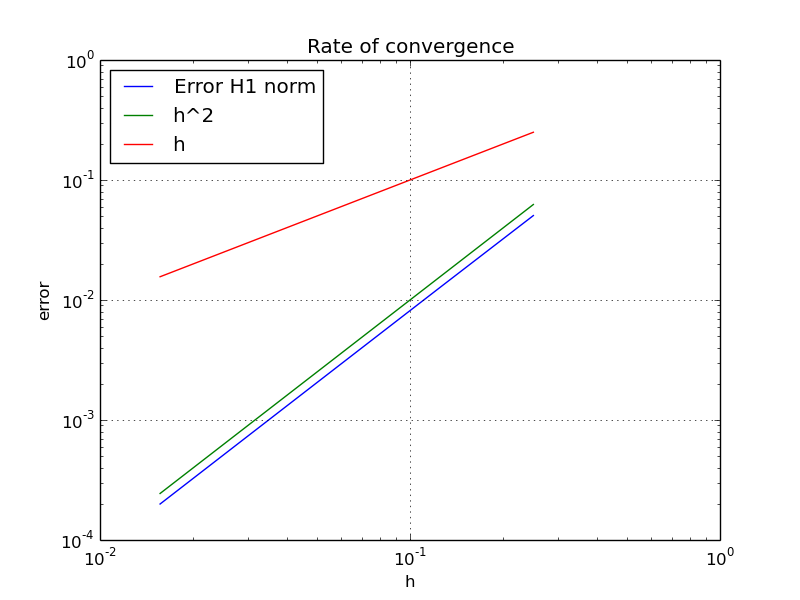
\includegraphics[width=\textwidth]{images/convergence_sine}
\caption{The plot shows a second order convergence, since the blue and green lines are parallel.}
\end{figure}
\vspace{1cm}

\begin{center}
\begin{tabular}{| c | c | c | c | c |}
\hline
$  \mathbf{N}$ & $ \mathbf{|| u_{exact} - u_h ||_{L^2}}$ & $  \mathbf{ | u_{exact} - u_h |_{H^1}}$ & \textbf{Rate in }  $ \mathbf{L^2}$ & \textbf{Rate in } $  \mathbf{H^1}$  \\
\hline
$ 4 $ & $1.9388 \times 10^{-3}$ & $5.0548 \times 10^{-2}$  & & \\
\hline
$ 8$ & $2.4515  \times 10^{-4}$ & $1.2733 \times 10^{-2}$ &  $2.9834$ &  $1.9890$   \\
\hline
$ 16 $ & $ 3.0745 \times 10^{-5}$ & $3.1896 \times 10^{-3}$ & $ 2.9952 $ & $1.9971$   \\
\hline
$ 32$ & $3.8465 \times 10^{-6}$ & $7.9780 \times 10^{-4}$ & $ 2.9987 $ & $ 1.9992 $  \\
\hline
$ 64$ & $4.8092 \times 10^{-7}$ & $1.9948 \times 10^{-4}$  & $ 2.9997 $ & $1.9998$ \\
\hline
\end{tabular}
\end{center}



\begin{center}
\begin{tabular}{| c | c | c |}
\hline
$\mathbf{N}$ & $\mathbf{|| p_{exact} - p_h ||_{L^2}}$ & \textbf{Rate in } $  \mathbf{L^2}$  \\
\hline
$ 4 $ & $1.4420  \times 10^{-4} $ & \\
\hline
$ 8 $ & $ 1.1896  \times 10^{-5} $ & $3.5995$ \\
\hline
$ 16 $ & $ 1.0089  \times 10^{-6} $ & $3.5596$ \\
\hline
$ 32 $ & $  8.7143 \times 10^{-8} $ & $3.5332$ \\
\hline
$ 64 $ & $ 8.0070 \times 10^{-9} $ & $3.4440$ \\
\hline
\end{tabular}
\end{center}




\section{Pressure-driven channel flow (2D)}
% References:
% Fenics book
% http://faculty.kfupm.edu.sa/CHE/usamah/CHE204/CHE204-HD22%20-%20Flow%20Through%20Circular%20Pipe.pdf

% Should I add some theory on this?

A typical test problem is finding the solution of the Navier-Stokes equations in a two-dimensional pressure-driven channel. We consider a viscous flow between parallel plates, where the geometry is the unit square $[0,1]^2$, and the kinematic viscosity is $\nu = 1/8$. We assume that both plates are fixed, i.e. no-slip boundary conditions are applied to the velocity at the upper and lower walls, and Neumann boundary conditions $\sigma \cdot \vec{n} = 0$ are applied at the inlet and outlet. Dirichlet boundary conditions are applied to the pressure at the inlet and outlet, with $p = 1$ at the inlet and $p = 0$ at the outlet. The initial condition for the velocity is $\mathbf{u} = (0,0)$. As a reference value in order to verify the agreement of our solution, we use the $x$-component of the velocity at the point $(x, y) = (1, 0.5)$ at final time $T = 0.5 $. The value reported on the FEniCS book [PUT REFERENCE] is $u_x(1, 0.5, T=0.5) \approx 0.44321183655681595$, while the one obtained in our results is $0.443217320106$.

\begin{figure}[h!]
\centering
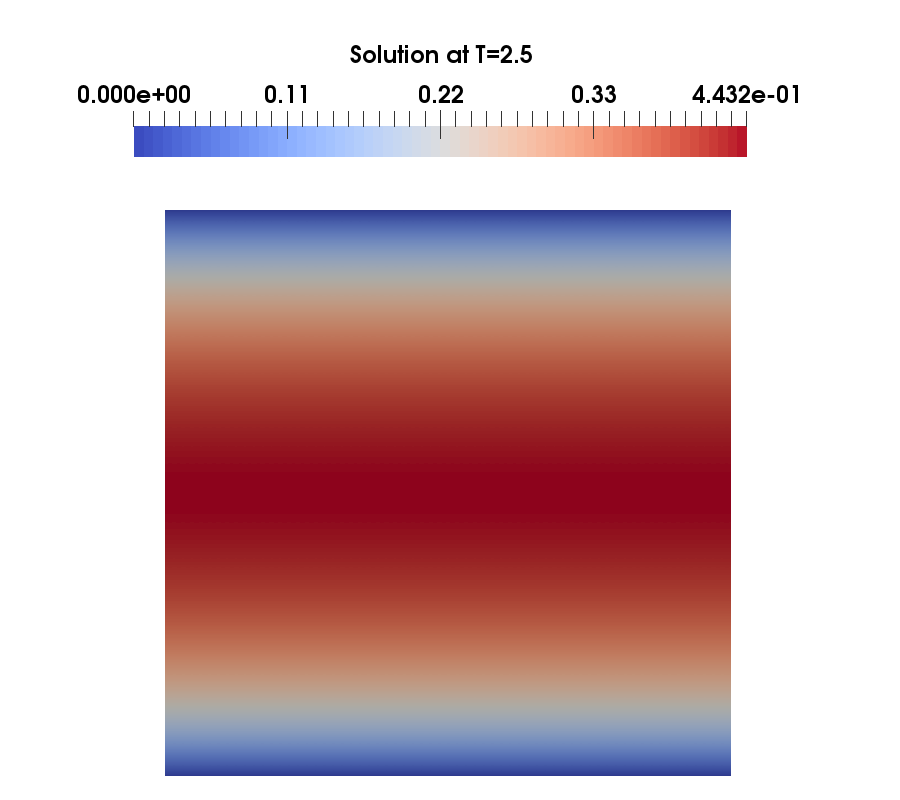
\includegraphics[width=0.8\textwidth]{images/velocity_solution.png}
\caption{The plot shows the solution $u(x,y)$ for $\nu = 1/8$.}
\end{figure}

\begin{figure}[h!]
\centering
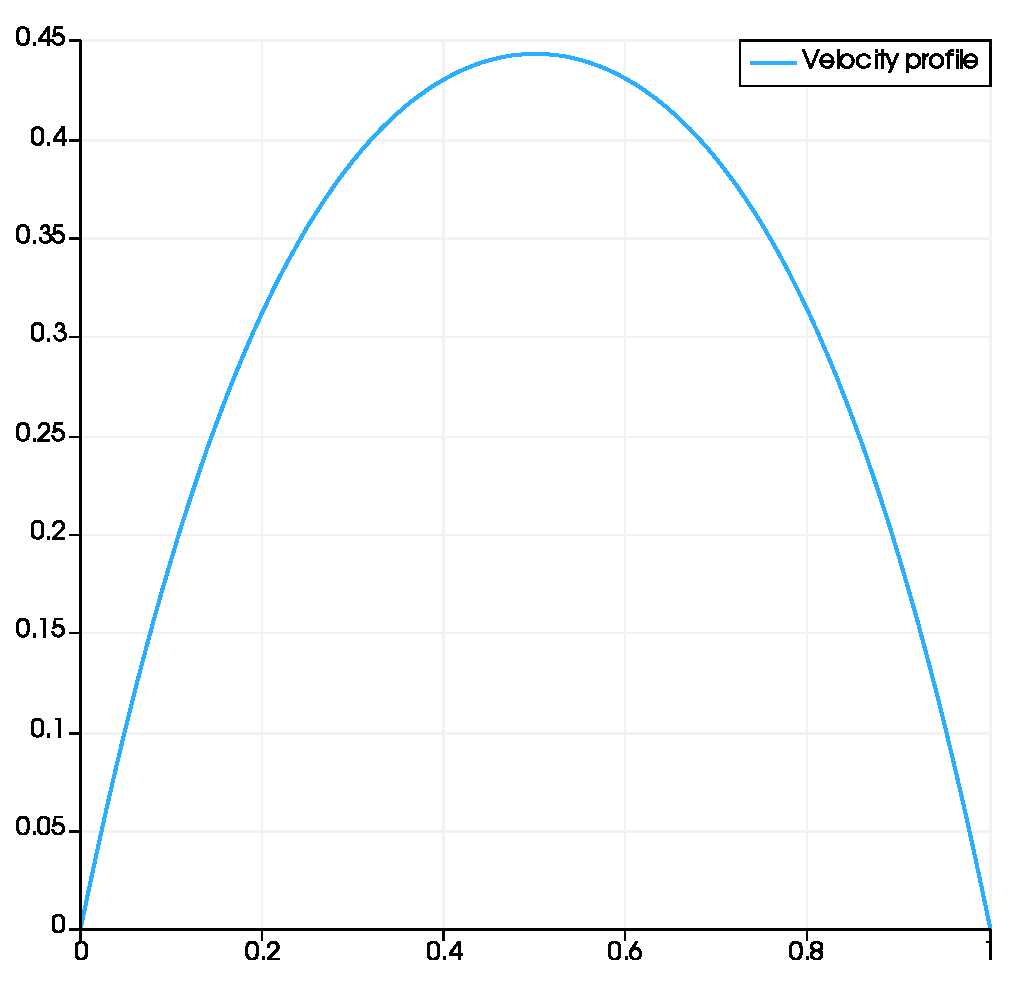
\includegraphics[width=0.6\textwidth]{images/velocity_profile.pdf}
\caption{Velocity profile at the points $(0.5, 1)$ and $(0.5, 0)$.}
\end{figure}

\section{Driven cavity}
% References:
% Fenics book, Quarteroni, Fluid dynamics F. White

A typical benchmark problem for fluid flow solvers in the two-dimensional lid-driven cavity problem. We consider a square cavity $\Omega$ with sides of unit length, i.e. $\Omega = [0,1] \times [0,1]$, kinematic viscosity $\nu = 1/1000$, and density $\rho = 1$. No-slip boundary conditions are imposed on each edge of the square, except at the upper edge where the velocity is set to $\mathbf{u} = (1,0)^T$, as follows

\[
\begin{cases}
\mathbf{u = 0}, & \mbox{on } \partial \Omega \backslash \Gamma \\
\mathbf{u} = (1,0)^T, & \mbox{on } \Gamma
\end{cases}
\]

where $ \Gamma = \set{ \mathbf{x} = (x,y)^T \in \partial \Omega | y = 1}$. We use finite elements on triangular grids of the type $\mathcal{P}_2-\mathcal{P}_1$. The initial condition for the velocity is set to zero. The resulting flow is a vortex developing in the upper right corner and then traveling towards the center of the square as the flow evolves. \\
To verify the correctness of the solver, we consider the minimum of the \textit{stream function}. The stream function $\psi$ allows us to satisfy the continuity equation and then solve the momentum equation directly for the single variable $\psi$. It is defined by

\[
\mathbf{u} = \nabla \times \psi = (\frac{\partial \psi}{\partial y} , - \frac{\partial \psi }{\partial x}),
\]

and it can be computed by solving the Poisson problem

\[
- \nabla^2 \psi = \omega,
\]

where $\omega$ is the vorticity given by

\[
\omega = \nabla \times \mathbf{u} = \frac{\partial u_y}{\partial x} - \frac{\partial u_x}{\partial y}.
\]


As a reference value, we use the one reported on the FEniCS book [REFERENCE], where the solution at the final time $T = 2.5$ was computed using the spectral element code Semtex with up to $80 \times 80$ $10^{th}$ order elements, heavily refined in the area in the vicinity of the minimum of the stream function. The time-stepping for computing the reference solution was handled by a third order implicit discretization, and a very short time step was used to minimize temporal errors.  The obtained reference value was $min(\psi) = -0.061 077$.

\begin{figure}[ht]
\centering
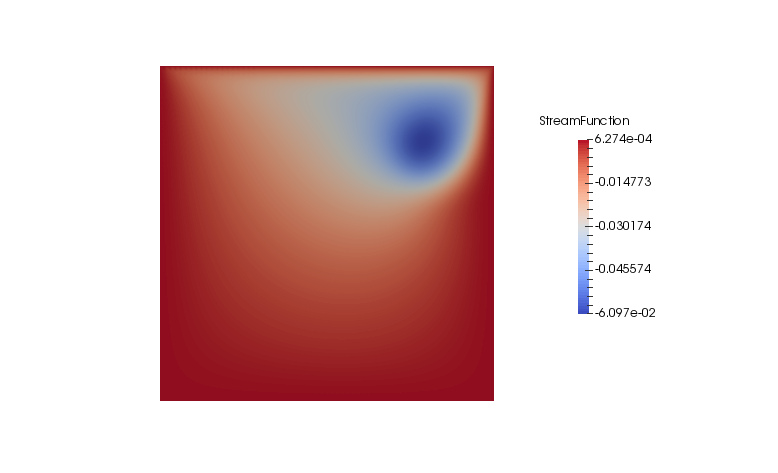
\includegraphics[width=\textwidth]{images/oyvind.png}
\vspace{-1cm}
\caption{The plot shows the stream function, and its minimum value $-0.06097$ (THIS IS OYVIND'S ).}
\end{figure}


In our case, a Crank-Nicolson (second order) discretization was used, with $\theta = 0.5$. A $64 \times 64$ number of elements was used, with $dt = 0.0125$ as time step. Hence, the obtained value was $min(\psi) = -0.061 121$, in fair agreement with the reference one. \\

\vspace{-.3cm}
\begin{figure}[ht]
\centering
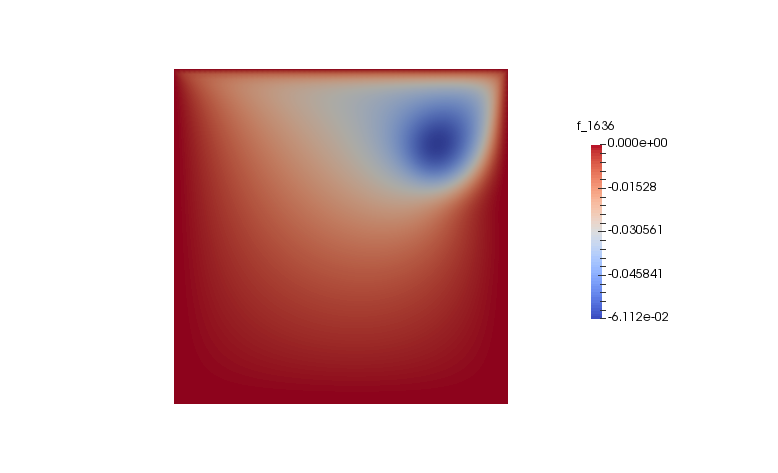
\includegraphics[width=\textwidth]{images/mine.png}
\vspace{-1cm}
\caption{The plot shows the stream function, and its minimum value $-0.061 121$.}
\end{figure}

(MISSING: PUT MY STREAM FUNCTION, OYVIND'S, AND THE ERROR BETWEEN THEM. \\
NOTE: Oyvind's stream function minimum is not exactly the same as the fenics book, what should I put then as a reference?)

\newpage

\section{MMS for Navier-Stokes and ALE}
As a test case for ALE we use the method of manifactured solutions. The exact solution that we choose has to satisfy the condition $\nabla \cdot \mathbf{u} = 0$. We can use the following functions

\begin{equation}
\mathbf{u}_{exact} = \left[ \begin{array}{c} sin(2\pi y) cos(2\pi x) cos(t) \\ - sin(2 \pi x) cos(2 \pi y) cos(t) \end{array} \right], \quad
p_{exact} = cos(x) cos(y) cos(t).
\end{equation}

Since in the N-S formulation with ALE we encounter also the mesh velocity $\mathbf{w}$, we need a $\mathbf{w}_exact$ which satisfies $- \Delta \mathbf{w}_{\rm exact} = 0$, as we are applying a Laplacian smoothing. We choose

\begin{equation}
\mathbf{w}_{exact} = \left[ \begin{array}{c} C \, sin(2 \pi y) cos(t) \\
0 \end{array} \right]
\end{equation}

As boundary conditions we choose

\begin{align}
\mathbf{u} &= \mathbf{u}_{exact} &&\text{on } \partial \Omega \setminus  \partial \Omega_{\rm tissue} \\
\sigma \cdot \mathbf{n} &= \sigma_{\rm exact} \cdot \mathbf{n} &&\text{on }  \partial \Omega_{\rm tissue}
\end{align}

where $\sigma_{\rm exact} = \mu \mathbf{u}_{\rm exact} - p_{\rm exact}I$.

The numerical scheme reads

\begin{equation}
\begin{split}
\rho \langle \frac{\mathbf{u}^{\rm i+1} - \mathbf{u}^{\rm i}}{\Delta t}, \mathbf{v} \rangle_\Omega
+ \rho \langle \nabla \mathbf{u}^{\rm i+ 1/2} \cdot (\mathbf{u}^i - \mathbf{w}^i), \mathbf{v} \rangle_\Omega
+ \mu \langle \nabla \mathbf{u}^{\rm i + 1/2} , \mathbf{v} \rangle_\Omega \\
- \langle p, div(v) \rangle_\Omega 
- \langle q, div(\mathbf{u}^{\rm i+1/2}) \rangle_\Omega
- \langle \sigma_{\rm exact} \cdot \mathbf{n}, \mathbf{v} \rangle_{\partial \Omega_{\rm tissue}} = \langle \mathbf{f}^{\rm i+1/2}, \mathbf{v} \rangle.
\end{split}
\end{equation}

\section{ALE + elasticity test case}

\chapter{Numerical results}

\chapter{Discussion}

\chapter{Conclusions}

\end{document}
